% Created 2024-10-18 Fri 03:45
% Intended LaTeX compiler: pdflatex
\documentclass[11pt]{article}
\usepackage[utf8]{inputenc}
\usepackage[T1]{fontenc}
\usepackage{graphicx}
\usepackage{longtable}
\usepackage{wrapfig}
\usepackage{rotating}
\usepackage[normalem]{ulem}
\usepackage{amsmath}
\usepackage{amssymb}
\usepackage{capt-of}
\usepackage{hyperref}
\usepackage{parskip,darkmode}
\enabledarkmode
\usepackage{tikz}
\author{Arnav Gupta}
\date{\today}
\title{Features And Constraints}
\hypersetup{
 pdfauthor={Arnav Gupta},
 pdftitle={Features And Constraints},
 pdfkeywords={},
 pdfsubject={},
 pdfcreator={Emacs 29.4 (Org mode 9.7.11)}, 
 pdflang={English}}
\begin{document}

\maketitle
\tableofcontents

\section{Constraint Satisfaction Problems}
\label{sec:orgf2fb812}
A CSP has:
\begin{itemize}
\item a set of variables
\item a domain for each variable
\item a set of constraints or evaluation function
\end{itemize}

Two kinds of problems:
\begin{enumerate}
\item \textbf{Satisfiability} Problems: find an assignment that satisfies constraints (hard constraints)
\item \textbf{Optimization} Problems: find an assignment that optimizes the evaluation function (soft constraints)
\end{enumerate}

A solution to a CSP is an assignment to the variables that satisfies all constraints (model of constraints).

CSPs can be represented as graph searching problems in two ways:
\begin{itemize}
\item \textbf{complete} assignment
\begin{itemize}
\item \uline{nodes}: assignment of value to all variables
\item \uline{neighbours}: change one variable value
\end{itemize}
\item \textbf{partial} assignment
\begin{itemize}
\item \uline{nodes}: assignment to first \(k-1\) variables
\item \uline{neighbours}: assignment to variable \(k\)
\end{itemize}
\end{itemize}

Search spaces can get large, so branching factors can be big.
Still, path to goal is not important, only the goal is.
No predefined starting node.

CSPs can be solved with:
\begin{itemize}
\item generate and test
\item backtracking
\item consistency
\item hill-climbing
\item randomized including local search
\end{itemize}
\subsection{Representations}
\label{sec:org462d42e}
\textbf{Primal} representations consider unary and binary constraints.
\textbf{Dual} representations consider N-ary constraints.
\subsection{CSP Solutions}
\label{sec:org7efa23a}
\textbf{Generate and Test}: go through all combos and check each one
\subsubsection{Backtracking}
\label{sec:orgba57656}
Prune large portions of the state space:
\begin{enumerate}
\item order all variables
\item evaluate constraints in the order as soon as they are grounded
\end{enumerate}

Efficiency depends on the order of variables, which can be hard to optimize.
Best to push failures as high as possible, since this cuts large branches of the tree early.
\subsubsection{Consistency}
\label{sec:orge28738a}
Look for inconsistencies through a graphical representation.
Specifically, give each domain a value until all constraints are satisfied.
\begin{enumerate}
\item Consistency Networks
\label{sec:org6dd8796}

\textbf{Domain constraint}: a unary constraint on values in a domain, written \(\left< X, c(X) \right>\).

A node in a consistency networks (CNs) is \textbf{domain consistent} if no domain value violates any domain constraint.
A CN is domain consistent if all nodes are domain consistent.

Arc \(\left< X, c(X, Y) \right>\) is a \textbf{constraint} on \(X\).
An arc \(\left< X, c(X, Y) \right>\) is \textbf{arc consistent} if \(\forall X \in D_{X}\), there is some
\(Y \in D_{Y}\) such that \(c(X, Y)\) is satisfied.
A CN is arc consistent if all arcs are arc consistent.

A set of variables \(\{ X_{1}, X_{2}, X_{3}, \dots, X_{N} \}\) is \textbf{path consistent} if all arcs
and domains are consistent.
\end{enumerate}
\section{AC-3}
\label{sec:orgcd028cc}
Makes a CN arc consistent and domain consistent with a \textbf{To-Do Arcs} (TDA) queue that has all inconsistent arcs.

\textbf{Algorithm}:
\begin{enumerate}
\item make all domains domain consistent
\item put all arcs \(\left< Z, c(Z, \_) \right>\) in TDA
\item repeat the following until TDA is empty
\begin{enumerate}
\item select and remove an arc \(\left< X, c(X, Y) \right>\) from TDA
\item remove all values of the domain of \(X\) that don't have a value in the domain of \(Y\) that satisfies
the constraint \(c(X, Y)\)
\item if any were removed, add all arcs \(\left< Z, c'(Z, X) \right>\) to TDA \(\forall Z \ne Y\)
\end{enumerate}
\end{enumerate}

AC-3 is guaranteed to terminate with one of:
\begin{itemize}
\item every domain is empty: no solution
\item every domain has a single value: solution
\item some domain has more than one value: split into two, run AC-3 recursively on each half
\end{itemize}

AC-3 has time complexity \(O(cd^{3})\) where \(c\) is the number of binary constraints and \(d\) is the maximum
size of each domain.
\section{Variable Elimination}
\label{sec:org5e706fd}
Eliminate the variables one by one, passing their constraints to their neighbours.
When a single variable remains, if it has no variables, the CN is \textbf{inconsistent}.
Variables are eliminated according to some elimination ordering.

\textbf{Algorithm}:
\begin{itemize}
\item if there is only 1 variable, return the intersection of the unary constraints that contain it
\item select a variable \(X\)
\begin{itemize}
\item join the constraints in which \(X\) appears, forming constraint \(R\)
\item project \(R\) onto its variables other than \(X\): call this \(R_{2}\)
\item place \(R_{2}\) between all variables that were connected to \(X\)
\item remove \(X\)
\item recursively solve the simplified problem
\item return \(R\) joined with the recursive solution
\end{itemize}
\end{itemize}
\section{Local Search}
\label{sec:org48dc29d}
\textbf{Steps}:
\begin{itemize}
\item maintain an assignment to each variable
\item at each step, select a neighbour of the current assignment
\item terminate when a satisfying assignment is found, or return the best assignment found
\end{itemize}

The aim is to find an assignment with no unsatisfied constraints (no conflicts).
So, the heuristic to be minimized is the number of conflicts.
\subsection{Greedy Descent}
\label{sec:org807aa01}
Goal is to find the variable-value pair that minimizes the number of conflicts at each step.

\begin{center}
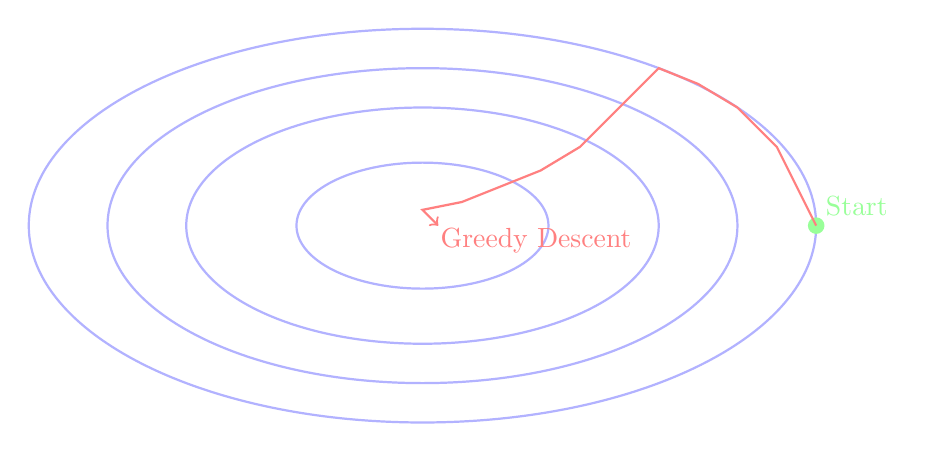
\begin{tikzpicture}

    % Outermost ring
    \draw[blue!30, thick] (0, 0) ellipse (5 and 2.5);

    % Second ring
    \draw[blue!30, thick] (0, 0) ellipse (4 and 2);

    % Third ring
    \draw[blue!30, thick] (0, 0) ellipse (3 and 1.5);

    % Innermost ring
    \draw[blue!30, thick] (0, 0) ellipse (1.6 and 0.8);

    % Starting point
    \fill[green!40] (5, 0) circle (3pt) node[above right] {Start};

    % Greedy descent path around the contours
    \draw[->, thick, red!50] (5, 0)
        -- (4.5, 1)
        -- (4, 1.5)
        -- (3.5, 1.8)
        -- (3, 2)
        -- (2.5, 1.5)
        -- (2, 1)
        -- (1.5, 0.7)
        -- (1, 0.5)
        -- (0.5, 0.3)
        -- (0, 0.2)
        -- (0.2, 0) node[midway, below right] {Greedy Descent};

\end{tikzpicture}
\end{center}

\textbf{Variants}:
\begin{itemize}
\item select variable in most conflicts and value that minimizes number of conflicts
\item select variable in any conflict and value that minimizes number of conflicts
\item select variable at random and value that minimizes number of conflicts
\item select variable and value at random
\end{itemize}

Problems can arise with finding:
\begin{itemize}
\item local minima rather than global minima
\item plateaus where heuristics are uninformative
\item ridges: local minima where looking ahead some number of steps may help
\end{itemize}

\textbf{Randomized Greedy Descent} allows for random steps (not just downward) and random restart
(reassign random values to variables).

In high dimensions, search spaces can have flat canyons that are hard to optimize.
\subsection{Stochastic Local Search}
\label{sec:orgc25d632}
Mix of greedy descent (move to lowest neighbour), random walk (take random steps), and random restart.
\subsubsection{Simulated Annealing}
\label{sec:orgd631a49}
\textbf{Steps}:
\begin{itemize}
\item pick a variable and new value at random
\item if it improves, adopt the new value
\item otherwise, adopt it probabilistically depending on temperature \(T\)
\begin{itemize}
\item with current assignment \(n\) and proposed assignment \(n'\), move to \(n'\) with probability
\(e^{-(h(n') - h(n))/T}\)
\end{itemize}
\item temperature can be reduced
\end{itemize}

High temperature \(\to\) higher probability of accepting a worse change.
\subsubsection{Tabu List}
\label{sec:org2e21d90}
To prevent cycling, maintain a \textbf{tabu list} of \(k\) last assignments and do not allow assignment
already on tabu list.

Can be implemented more efficiently than a list of complete assignments, but still expensive.
\subsubsection{Parallel Search}
\label{sec:org5212d48}
Total assignment called an \textbf{individual}:
\begin{itemize}
\item maintain a population of \(k\) individuals instead of one
\item at each stage, update each individual
\item whenever an individual is a solution, it can be reported
\item similar to using \(k\) restarts but uses \(k\) times the minimum number of steps
\end{itemize}
\subsubsection{Beam Search}
\label{sec:orgec2dfb7}
Like parallel search, but choose the \(k\) best out of all neighbours.
\begin{enumerate}
\item Stochastic Beam Search
\label{sec:org7dcae53}
Probabilistically choose the \(k\) individuals at the next generation, using the heuristic:
\(e^{-h(n)/T}\).

Maintains diversity and heuristic reflects fitness.
\end{enumerate}
\subsubsection{Genetic Algorithms}
\label{sec:org393f114}
Pairs of individuals combine to create offspring:
\begin{itemize}
\item randomly choose pairs of individuals where the fittest are most likely to be chosen
\item for each pair, perform a \textbf{cross-over}: form offspring taking parts of the parents
\item mutate some values
\end{itemize}
\subsection{Comparing Stochastic Algorithms}
\label{sec:org7fcc2bc}
\textbf{Runtime Distribution}: plot runtime and proportion of runs that are solved in that runtime
\end{document}
